\chapter{Introduction}
\label{chapter:intro}
\epigraph{Don’t be scared. All of this is new to you, and new can be scary. Now we all want answers. Stick with me---you might get some.}{\textit{The 13th Doctor} - Doctor Who}

Static program analysis is the cornerstone of several modern programming facilities and tools for program development and aided program understanding. Nowadays, it is an umbrella term for many different methodologies (\todo{}) all with the ultimate goal of inferring a program's properties, without the need of an actual execution. It is routinely employed in many different contexts: compilers, bug detectors, verifiers, security analyzers, IDEs, and a myriad other tools.

The main intention of any \emph{static} program analysis algorithm is to reason about the set of all feasible behaviors (under some abstraction of behaviors) that a given program might exhibit under all possible executions. For example, could this method throw a runtime exception? or is that type cast possible to fail under some program input? etc. Subsequently, virtually all interesting static program analysis questions are undecidable---indeed the prototypical undecidable problem, the \emph{halting problem}, is a static program analysis question: will a program terminate under all inputs?

Pointer analysis (also known as \emph{points-to analysis}) is a fundamental subdomain of static program analysis that consists of computing some \emph{abstract memory model} for a given program. The essence of such an analysis is to compute a set of possible objects that a program variable or expression may point to during program execution. A straightforward endeavor at first, it quickly gets too complicated in practice due to all of the intricate details one has to take into account and the multitude of different features that mutually depend on each other.\footnote{The analysis inputs are large and the analysis algorithms are typically quadratic or cubic, but try to maintain near-linear behavior in practice, by exploiting program properties and maintaining precision---more precise (i.e., smaller) inference sets lead to less work.} Although a challenging task, smart implementations of pointer analysis can bear many benefits to client analyses that will subsequently consume the results to reason about specialized behaviors (e.g., security vulnerabilities or potential optimization opportunities).

A closely related analysis, sometimes wrongfully confused with pointer analysis, is \emph{alias analysis} in which one computes sets of program expressions that may alias (i.e., point to common objects) with each other. Pointer analysis could---although it is not the only possible alternative---be used to implement an alias analysis algorithm, and vice versa.

At the same time, programming languages are ever evolving, ever becoming higher-level and more complex. Many abstraction levels are added throughout the years with the aim of making the very task of programming easier for developers allowing them to express more with less effort (e.g., in terms of lines of code). Frequently, new features come with complicated semantics regarding their possible implementations and usually they interact in intricate ways with pre-existing ones.

Additionally, modern software paradigms have evolved as well. Complex design patterns have become the norm for experienced developers, immense libraries and frameworks are accepted as a prerequisite for any non-trivial software, and over-involved build tools often make even the task of understanding all of the program's dependencies a challenge.

It comes as no surprise that any kind of static analysis has struggled to keep up with this ever-increasing complexity both in programming languages and software. Even the seemingly simple task of computing a program's call-graph (i.e., which methods are called at every invocation site) requires sophisticated analysis for achieving acceptable precision. Thus, the main emphasis of pointer analysis algorithms is on combining fairly precise modeling of pointer behavior and memory abstractions with scalability.

%\paragraph*{Thesis.}
%\begin{displayquote}
%It is possible to implement \emph{highly sophisticated} and \emph{precise} static pointer analysis algorithms without forgoing \emph{scalability}. Furthermore, precision and the accompanied \emph{confidence in results} is a spectrum and can be tweaked differently for different parts of the program.
%\end{displayquote}

\paragraph*{Thesis}
\begin{displayquote}
It is possible to implement \emph{highly sophisticated} and \emph{precise} static pointer analysis algorithms without forgoing \emph{scalability}. Furthermore, precision and the accompanied \emph{confidence in results} is not a global property of a given algorithm, but can be tweaked differently for different parts of the program.
\end{displayquote}

We provide a number of techniques for implementing scalable static pointer and alias analyses in the setting of Java programs by configuring the analysis strategy differently for different code parts. Additionally, we present a couple of defensive algorithms for reporting high-confidence results even in the presence of hostile or unknown program points.


\section*{Background}
There are a few important design choices that can affect drastically the properties a static program analysis algorithm will enjoy and the reasoning that is required to achieve such goals. A bird's-eye view is given below.

\section{Context Sensitivity}

Throughout the years, pointer analysis has evolved and has been the focus of intense research. It is widely accepted to be among the most standardized and well-understood inter-procedural (i.e., reasoning about a property taking into account the flow of code across different program functions) analyses.

The emphasis of points-to analysis algorithms is on combining fairly precise modeling of pointer behavior with scalability. The challenge is to pick judicious approximations that will allow satisfactory precision at a reasonable cost. Furthermore, although increasing precision often leads to higher asymptotic complexity, this worst-case behavior is rarely encountered in actual practice. Instead, techniques that are effective at maintaining good precision often also exhibit better average-case performance, since smaller points-to sets lead to less work.

A widely used concept that emerged as a powerful tool for tuning precision while still achieving scalable analyses, is that of \emph{context-sensitivity}. It consists of qualifying interesting components of an analysis, such as program expressions, object abstractions or method invocations, with additional \emph{context} information. The core idea being that the analysis will collapse information (e.g., ``what objects this method argument may point to'') for executions that result in the same context, while keep separate information for different contexts. In essence, qualifying components with additional context is as if each such component is replaced with multiple versions (one for each different associated context value) and the analysis can reason individually for each version. This approach tries to counter the loss of precision that naturally arises in any static analysis, from conflating information of different dynamic program paths.

Two main flavors of context sensitivity have been explored in past literature:
\begin{inparaenum}[(1)]
\item \emph{call-site sensitivity} (also known as \emph{$k$CFA}) \cite{col:1981:Sharir,thesis:Shivers} in which call-sites are used to qualify variables and other analysis components, essentially re-analyzing a method for different call-sites that target that method, and
\item \emph{object-sensitivity} \cite{issta:2002:Milanova,article:2005:Milanova,popl:2011:Smaragdakis} in which receiver objects of a call are used instead, in a similar manner.
\end{inparaenum}
Another kind of context sensitivity, known as \emph{type-sensitivity}, has also been explored as an approximation of object sensitivity with the aim of preserving high precision at substantially reduced cost. In type sensitivity, upper bounds on the dynamic types of the receiver objects are employed as context elements.

A context-sensitive analysis has a second axis of parameterization besides context flavor---that of (max) context depth. Consequently, a common way to describe an analysis is using the following naming scheme: $X$-FLAVOR-sensitive+$Y$-heap, e.g., as in 3-call-site-sensitive+2-heap. Here FLAVOR denotes the kind of context information being employed, and, $X$ and $Y$ denote the context depth limits being used at invocation sites and at object allocations respectively. In the previous example the analysis is keeping track of the 3 most recent call-sites that led to the current method call, in order to annotate local variables. Similarly, the analysis is using the 2 most recent call-sites that led to the allocation site of an object to annotate the newly allocated object.


\subsection{Call-Site Sensitivity (\texorpdfstring{$k$}{k}CFA)}

As previously mentioned, a call-site sensitive analysis uses method call sites (i.e., labels of invocation instructions) as context elements. The analysis separates information on program expressions, such as local variables, per call-stack (i.e., sequence of $k$ most recent call-sites) that led to the current method call. Similarly, the analysis separates information on heap objects per call-stack that led to the object's allocation.

For instance, in the code snippet of Figure~\ref{fig:hybrid:snippet}, a \emph{1-call-site-sensitive} analysis (unlike a \emph{context-insensitive} analysis) will distinguish the two call-sites of method \code{foo} in lines 7 and 9. This results in an analysis that will treat \code{foo} separately in two cases: that of its formal argument, \code{arg}, pointing to anything \code{obj1} may point to, and that of \code{arg} pointing to anything \code{obj2} may point to.

An equivalent mental model is that of two instances of method \code{foo} being analyzed---\code{foo\_COPY1} and \code{foo\_COPY2}. The invocation in line 7 leads to \code{foo\_COPY1}, whereas the one in line 9 leads to \code{foo\_COPY2}. After the analysis has been concluded, if one is to query regarding method \code{foo}, information from both instances will be collapsed into as single answer-set.

\begin{figure}[htp]
\begin{javacode}
class A {
    void foo(Object arg) { ... }
}

class B {
    void bar(A a1, A a2) {
        ...
        a1.foo(obj1);
        ...
        a2.foo(obj2);
    }
}
\end{javacode}
\caption{Code snippet for illustrating context-sensitive analyses.}
\label{fig:hybrid:snippet}
\end{figure}

\subsection{Object Sensitivity}

In contrast, an object sensitive analysis uses allocation sites (i.e., labels of instructions containing a \code{new} statement) as context elements. (Hence, a better name for ``object-sensitivity'' might have been ``allocation-site sensitivity''.) When a method is called on an object (also known as the call \emph{receiver}), the analysis separates information depending on the allocation site of that object, as well as other, previous allocation sites used as context.

Thus, in the code of Figure~\ref{fig:hybrid:snippet}, a \emph{1-object-sensitive} analysis will analyze \code{foo} separately on all the allocation sites of objects that \code{a1} and \code{a2} may point to. If, for example, \code{a1} and \code{a2} are inferred to potentially point to objects from two and three distinct allocation sites respectively, \code{foo} will effectively be analyzed under five different contexts. On the other hand, if the analysis has inferred that both \code{a1} and \code{a2} may only point to objects from a single common allocation site, then the method will only be analyzed under one context.

It is not apparent from this code fragment---and this also holds in the general case--neither whether \code{a1} and \code{a2} may point to different objects, nor to how many: the allocation site of the receiver object may be remote and unrelated to the method call itself. Similarly, it is not possible to compare the precision of an object-sensitive and a call-site-sensitive analysis in principle. In this example, it is not even clear whether the object sensitive analysis will examine all calls to \code{foo} as one case, as two, or as many more, since this depends on the allocation sites of all objects that the analysis \emph{itself} computes to flow into \code{a1} and \code{a2}.


\section{Intraprocedural vs. Interprocedural Analyses}

Different kinds of static program analysis may define differently which program parts are of interest. An \emph{intraprocedural} analysis makes its reasoning using only the local information that is available in each program function. Multiple analyses commonly found in a classical compiler, such as \emph{type-checking} or the computation of \emph{live-ranges} for program variables are well-known examples of intraprocedural static program analyses. On the contrary, an \emph{interprocedural} analysis is one whose reasoning transcends function boundaries, taking into account how different functions interact with each other. An analysis reasoning about \emph{thrown exception}---that flow out of a function---is one such example.

Furthermore, a related categorization is that of a \emph{whole-program} analysis in contrast to a \emph{modular} one. A whole-program analysis examines every part of the program, including any external dependencies that the code may have, and reasons about the effects each part has on the rest of the program. In the setting of Java, for example, a whole-program analysis not only reasons about the application code but additionally about any third-party library used by the program (e.g., from external Java Archives---JARs) and also about code run by the Java Runtime Environment---i.e, library code provided by the language itself. On the other hand, a modular analysis only focuses on specific parts of the program and ignores the effects of the rest (e.g., an analysis focusing on certain Java packages).

A modular analysis usually may afford to implement more complex, more expensive reasoning than a whole-program one, since it only focuses on a very localized part of the program. On the contrary, a whole-program analysis has to constantly balance the complexity of its logic,  any potential precision gains but also any scalability penalties. The rest of this dissertation will only focus on a few interesting whole-program analyses.


\section{Flow-Sensitivity}
\label{sec:intro:flowSensitivity}

Although counter-intuitive at first, it is not unusual for a static program analysis to be flow-\emph{insensitive}. A flow-sensitive analysis examines a method's instructions while taking into account the order they appear in the source code. On the contrary, a flow-insensitive analysis examines a method's instructions as if they were in a set, without any particular order (i.e., any instruction could happen before any other), and as if they may repeat any number of times. The latter approach leads to analyses that overapproximate the semantics of the actual code---thus potentially suffering in precision---but it is a common tradeoff when aiming to improve the performance of an analysis.

The penalties on performance for a flow-sensitive analysis mainly stem from the need to keep track of what holds at \emph{every single} program point. Potentially, this could mean that information that remains unchanged will be duplicated on a multitude of instructions. On the contrary, a flow-insensitive analysis will collapse information along all instructions of a method.

{
\setlength\intextsep{-10pt}
\begin{wrapfigure}{ht}{.12\textwidth}
\centering
\begin{javacode}
x = 1;
y = x;
x = 2;
\end{javacode}
\end{wrapfigure}

For the example on the side, a flow-sensitive analysis reasoning about the values of primitive expressions might report that:
after line 1: ``$x$ has the value 1'',
after line 2: ``$x$ has the value 1'' and ``$y$ has the value 1'', and
after line 3: ``$x$ has the value 2'' and ``$y$ has the value 1''.

A flow-insensitive analysis might instead report that:
``$x$ has either the value 1 or 2'' and ``$y$ has either the value 1 or 2'',
because instructions are examined as if happening in any order.
}


\section{Static Single Assignment Form}
\label{sec:intro:ssa}

In compiler design, \emph{static single assignment form} (also known as SSA) is a kind of code transformation in which every local variable is assigned only once. Existing local variables in the original source code are split into \emph{versions} (e.g., variable $x$ might be split into $x_1$ and $x_2$) with each version being assigned only once. At program points where the value of the original variable is read and there are multiple valid versions, as in the point where the branches of an \emph{if-else} statement merge, a \emph{phi-node} statement is used. This special statement bears the semantics of somehow ``choosing'' a specific variable version to read.

\begin{figure}[h]
\begin{subfigure}{.45\textwidth}
\begin{javacode}
if (...) x = 10;
else x = 20;
y = x;
\end{javacode}
\caption{Original source code}
\end{subfigure}%
\hfill
\begin{subfigure}{.45\textwidth}
\begin{javacode}
if (...) x_1 = 10;
else x_2 = 20;
y = phi(x_1, x_2);
\end{javacode}
\caption{The equivalent SSA form}
\end{subfigure}
\caption{Example code before and after an SSA transformation}
\end{figure}

In the context of static program analysis, SSA is often used to approximate the benefits of a flow-sensitive analysis, particularly pertaining to the handling of local variables. This is not the case for other, more complicated language features such as heap accesses and method invocations, but SSA provides an easy way to pick the low-hanging fruit.

\setlength\intextsep{15pt}
\begin{wrapfigure}{ht}{.12\textwidth}
\centering
\begin{javacode*}{xleftmargin=10pt,linenos=false}
x_1 = 1;
y = x_1;
x_2 = 2;
\end{javacode*}
\end{wrapfigure}

The flow-\emph{insensitive} analysis of \ref{sec:intro:flowSensitivity} will report quite different results when analyzing the SSA-form analogue of the example code (given on the side): ``$x_1$ has the value 1'', ``$y$ has the value 1'', and ``$x_2$ has the value 2''. The analysis is still examining instructions without taking order into account, and is unable to answer questions such as ``what is the value of variable $x$ at the end of the method'' (whether the value of $x_1$ or $x_2$ is the final one), but nevertheless it has managed to reclaim some of the precision that was previously lost---i.e., regarding the value of variable $y$.


\section{May vs. Must Analyses}
\label{sec:intro:may-must}

Given an abstraction of behaviors (e.g., thrown exceptions) one can define two interesting sets regarding the potential behaviors that a given program will exhibit. Set $Any(P)$ is defined as containing all possible behaviors that a program $P$ \emph{will} exhibit in \emph{some} program execution (e.g., method $m1$ will throw exception $e1$ in one execution and exception $e2$ in another). Respectively, set $All(P)$ is defined as containing behaviors that will appear in \emph{every} program execution (e.g., method $m2$ will always throw exception $e3$ during any execution).
\[
Any(P) := \bigcup_{e \in Executions} Behaviors(P, e)
\quad \textrm{and} \quad
All(P) := \bigcap_{e \in Executions} Behaviors(P, e)
\]

Both sets are a mathematical ideal, an answer only an oracle could provide. But, for any realistic analysis such an endeavor is an undecidable problem. Thus, a practical static program analysis will aim to compute an approximation of one of the two sets. Under that definition, analyses are split mainly into two groups depending on the kind of approximation they try to achieve. On one hand, a \emph{may}-analysis is one that aims to \emph{over}-approximate $Any(P)$. On the other hand, a \emph{must}-analysis is one that aims to \emph{under}-approximate $All(P)$.
\[
May(P) \supseteq Any(P) \quad \textrm{and} \quad Must(P) \subseteq All(P)
\]

For the rest of this dissertation, unless otherwise noted, all described analyses aim to compute $May(P)$, i.e., they are may analyses. This also reflects the fact that may analyses comprise the norm in related literature.


\section{Soundness \& Completeness}
\label{sec:intro:soundness}

The term \emph{soundness}, and its converse \emph{completeness}, originate from formal mathematical logic where they are used in order to evaluate a \emph{proof} system under a given \emph{model}. The model is some kind of mathematical structure, such as sets over some domain of interest and the proof system is a set of rules with which \emph{properties} regarding the model are proven. A system is sound if and only if statements it can prove are indeed true in the model (concisely given as ``claim implies truth''). A system is complete if and only if what is true in the model can also be proven by the system (concisely given as ``truth implies claim'').

In the context of static program analysis, the most relevant and widely used term is that of soundness. In this setting, the analysis is making claims regarding potential program behaviors under any program execution and the validity of those claims constitutes whether the analysis is sound or not. More specifically, a may-analysis is sound whenever what it claims is actually true---i.e., the computed behaviors are an overapproximation of $Any(P)$. Respectively, a must-analysis is sound whenever the computed behaviors are an underapproximation of $All(P)$. A trivially sound-may analysis could simply infer top ($\top$), i.e., every possible behavior. A trivially sound-must analysis could simply infer the empty set ($\emptyset$), i.e., no behavior at all.

Contrary to the prevalent use of soundness for evaluating static program analysis algorithms, completeness is scarcely referenced---if ever. One can easily find ``proofs of soundness'' on many publications but not the analogous ``proofs of completeness''. This is mainly because of the way analyses (may- or must-) are defined as aiming to compute an \emph{approximation} of potential behaviors. For example, what would the meaning of a complete may-analysis be? Such an analysis has to abide by the definition of ``truth implies claim''. In this case ``truth'' is any overapproximation of $Any(P)$. Consequencently, a ``complete'' may-analysis would need to compute all possible overapproximations of $Any(P)$, and thus, the term is less relevant in the domain of static program analysis.

Relatedly to soundness, there are two closely related terms characterizing the validity of each claim made by the analysis. If the analysis incorrectly claims that some behavior is among the potential program behaviors, then this constitutes a \emph{false-positive}. E.g., if the analysis claims that method $m1$ might throw an exception $e1$, but there is no program execution under which this will actually occur. Similarly, if an analysis claims that some behavior will never happen but in reality there exists a program execution where such a behavior takes place, then this constitutes a \emph{false-negative}. E.g., if the analysis claims that method $m2$ will never throw an exception, but it actually does. By consequence of previous definitions, a sound may analysis will make no false-negative claims, and a sound must analysis will make no false-positive ones.

It is noteworthy that every static program analysis is also making negative claims, in addition to positive ones, even if only implicitly. This is due to an analysis not making some claim actually implicitly claiming its negation. For example, if a may-analysis for thrown exceptions reports that method $m1$ might throw either exception $e1$ or exception $e2$, then it also implicitly reports that the same method will never throw any other exception---given that the analysis aims to compute an overapproximation of possible behaviors.


\section{Precision \& Recall}
\label{sec:intro:precision-recall}

Both a may- and a must-analysis operate under the premise of computing an approximation of reality and thus there will always be claims that are either extraneous or missing. Of course, any analysis should do its best to get as close to the truth, even if the actual set of behaviors will always be out of grasp. This calls for some \emph{quantitative} way to measure an analysis's quality. Two such metrics have been proposed. \emph{Precision} indicates how many of the analysis claims are actually part of the truth, whereas \emph{recall} indicates how many of the actual true claims are also reported by the analysis. For a formal definition supposing that:
\begin{itemize}
\item $X$ is the number of true (actually happening) interesting behaviors
\item $T \leq X$ is the number of correct claims made by the analysis (the \emph{true-positives})
\item $F$ is the number of incorrect claims made by the analysis (the \emph{true-negatives})
\end{itemize}
then
\[
Precision(P) = \frac{T}{T + F}
\quad \textrm{and} \quad
Recall(P) = \frac{T}{X}
\]

A value of 1 is a perfect score, and a value of 0 is the worst one. A sound-may analysis will have perfect recall, since it at least claims any behavior that is actually true. A sound-must analysis will have perfect precision, since it makes no incorrect claims (it does not report any behavior that cannot actually occur).

Highly useful as they are, both measures have a major, unavoidable shortcoming. It is rarely the case that there is actual knowledge of the ground-truth. Somewhat a chicken-and-egg problem, having an automatic way to retrieve the ground-truth for arbitrary programs is both what a static analysis aims to achieve at its core and also what is needed to evaluate its claims. Usually, one has to resort to observing a limited amount of actual executions for a given program and---making the assumption that the observations are a good enough representative---interpolate to all possible program executions.

Furthermore, this approach makes both measures \emph{empirical}, in the sense that they measure an analysis's performance in regards to a \emph{specific} given program. They bear no information in regards to the analysis behavior at a theoretical level and cannot be generalized to other programs. An analysis could be perfect for one program and terrible for another. This could be tackled to some extent with the use of well-established \emph{benchmarking suites} during the testing phase, that aim to cover common and interesting code patterns and program behaviors.


\section{Soundiness}

Although soundness seems like an essential property for any static program analysis algorithm to have, and is quite prevalent in academic literature, Livshits et al (\todo{}) make a strong claim that there is no practical sound \emph{whole-program} may-analysis. Most of the time, this is a conscious compromise on how to handle certain language features and not due to lack of understanding. If one would attempt to soundly model such features in the context of a may-analysis, i.e., overapproximate their effects, this would most probably result in an analysis that is so unscalable or imprecise that is practically \emph{useless}.

At the same time, many academic publications make claims of soundness and may even provide some kind of ``proof of soundness'' but this is mostly in regards to a \emph{subset} of language features---the analysis might be totally unsound in handling all the rest. Thus, a need arises for a way to differentiate between an analysis that tries its best to be sound and only gives up in a well-defined language subset, and one that is simply unsound.

The term \emph{soundiness}, specific to the context of static program analysis, was coined by (\todo{}) for such a purpose. A \emph{soundy} analysis handles most classical, core language features in a sound manner (i.e., overapproximates) and may only fail to do so (i.e., underapproximates) in a small well-accepted subset of highly \emph{dynamic features}, specific to each language. Such features include uses of \emph{reflection} or \emph{native code} in Java, \emph{eval} in Javascript, and \emph{pointer arithmetic} in C/C++.


\section{A Static Program Analysis Mind Map}

\begin{figure}[htb!]
\begin{subfigure}{.47\textwidth}
    
\includegraphics[scale=.45]{assets/introduction/venn-soundness-a.pdf}
    \caption{Behavior sets of actual program executions}
    \label{fig:intro:soundness-a}
\end{subfigure}
\hfill
\begin{subfigure}{.47\textwidth}
    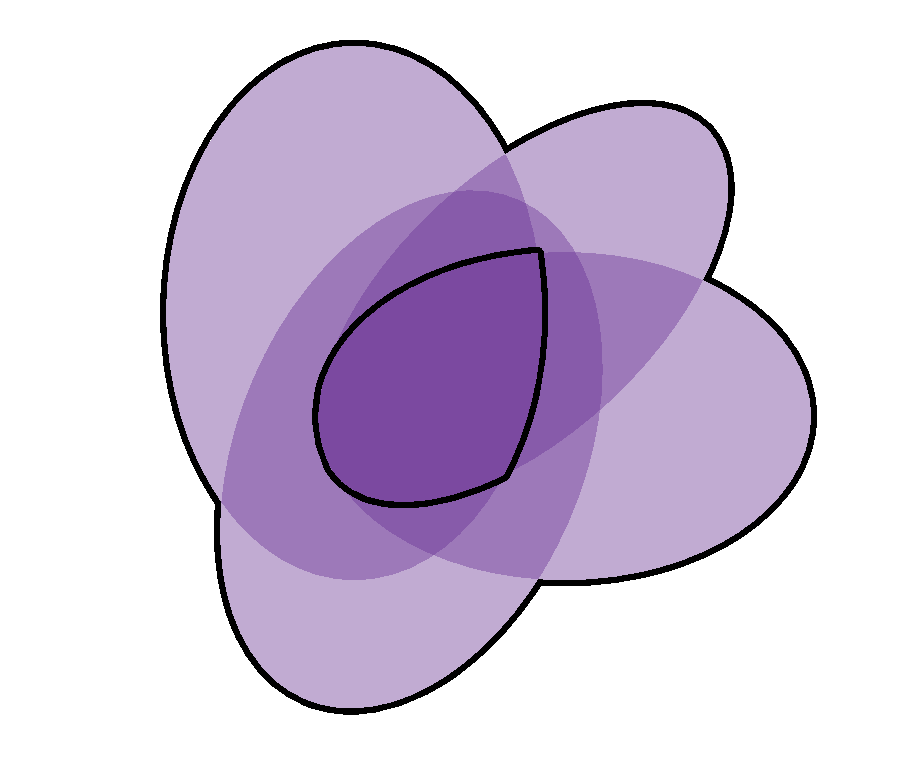
\includegraphics[scale=.45]{assets/introduction/venn-soundness-b.pdf}
    \caption{Mathematical ideals $Any(P)$ (union) and $All(P)$ (intersection)}
    \label{fig:intro:soundness-b}
\end{subfigure}
\begin{subfigure}{.47\textwidth}
    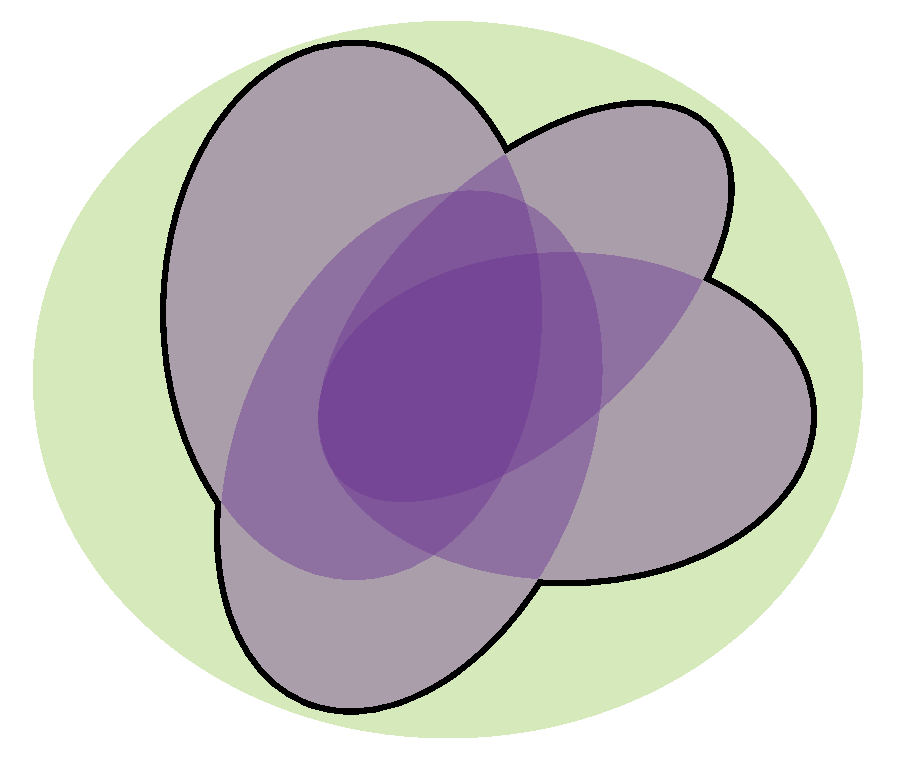
\includegraphics[scale=.45]{assets/introduction/venn-soundness-c.pdf}
    \caption{Any sound-may analysis (green) in relation to $Any(P)$}
    \label{fig:intro:soundness-c}
\end{subfigure}
\hfill
\begin{subfigure}{.47\textwidth}
    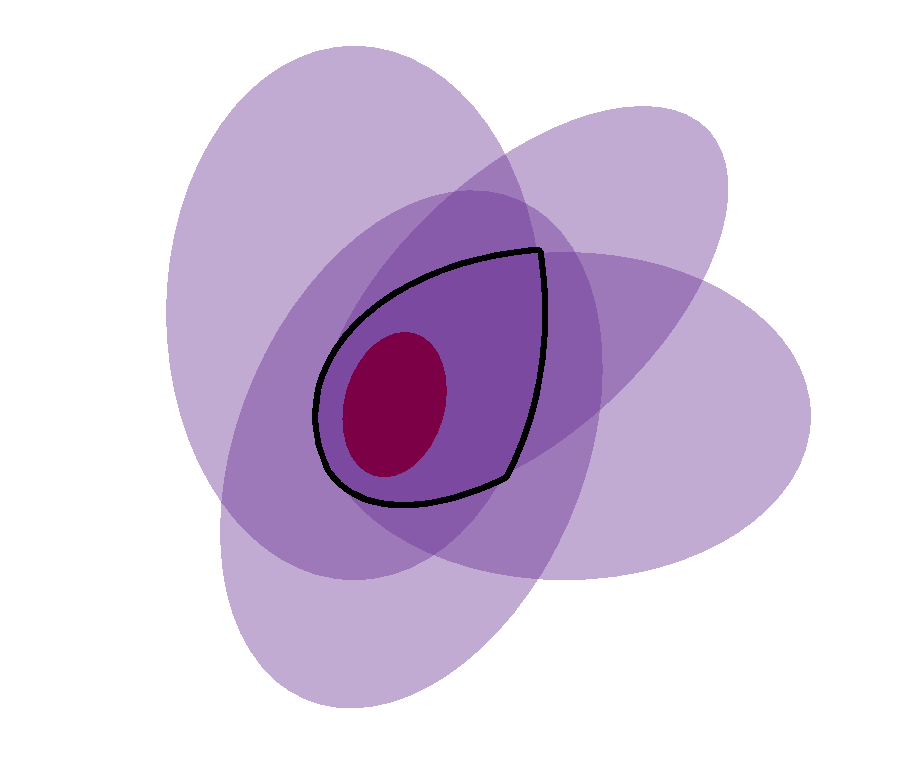
\includegraphics[scale=.45]{assets/introduction/venn-soundness-d.pdf}
    \caption{Any sound-must analysis (red) in relation to $All(P)$}
    \label{fig:intro:soundness-d}
\end{subfigure}
\begin{subfigure}{.47\textwidth}
    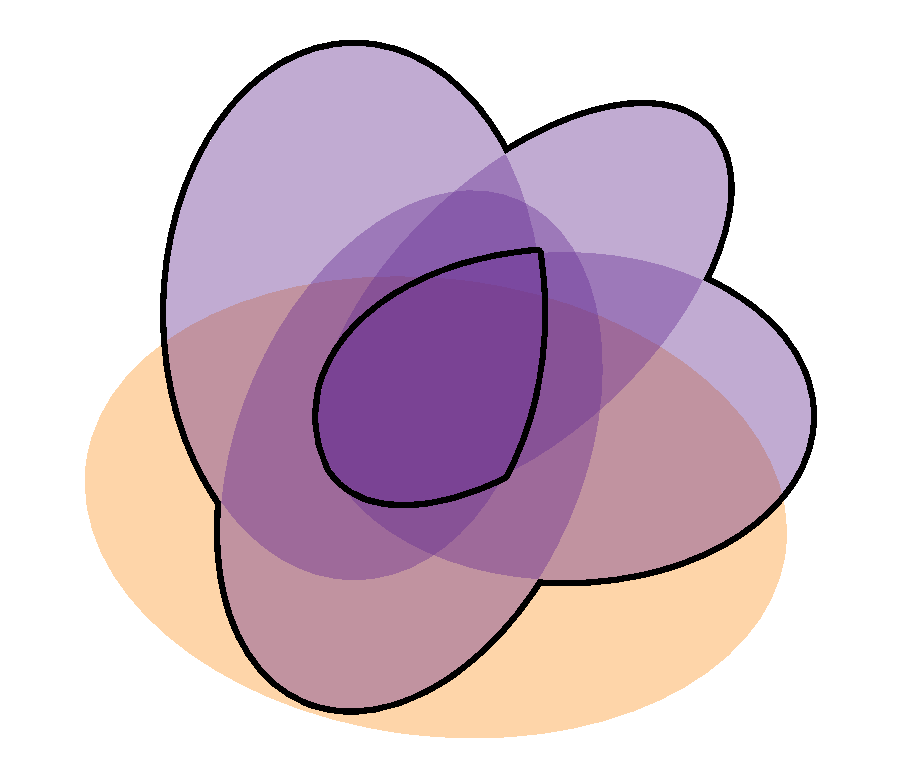
\includegraphics[scale=.45]{assets/introduction/venn-soundness-e.pdf}
    \caption{Any unsound analysis (orange) in relation to both ideals}
    \label{fig:intro:soundness-e}
\end{subfigure}
\hfill
\begin{subfigure}{.47\textwidth}
    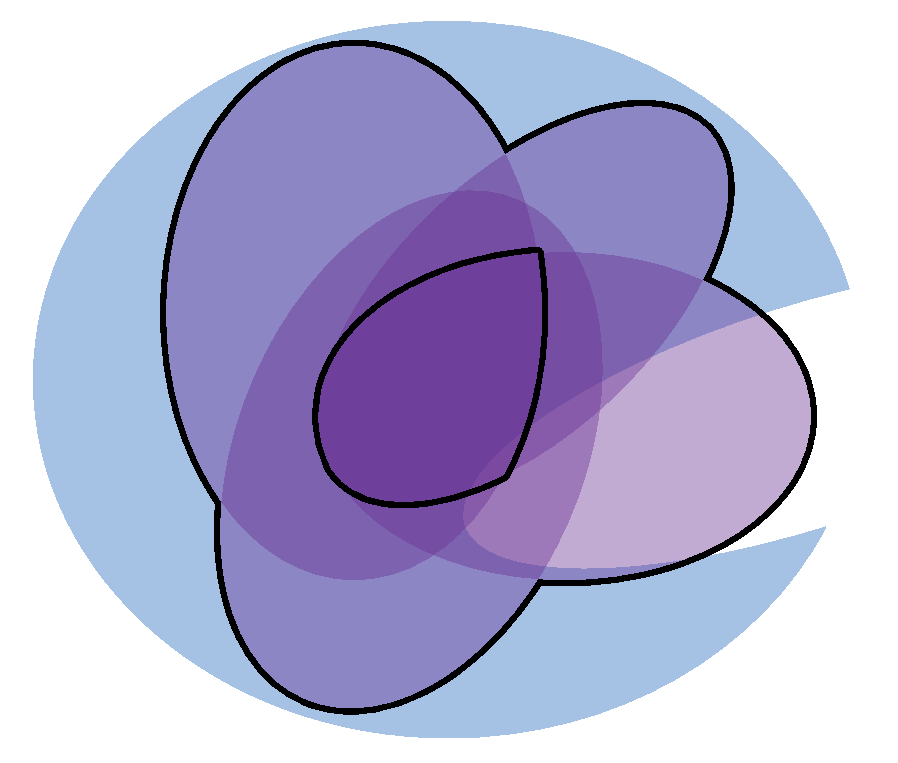
\includegraphics[scale=.45]{assets/introduction/venn-soundness-f.pdf}
    \caption{Any \emph{soundy} analysis (blue) in relation to both ideals}
    \label{fig:intro:soundness-f}
\end{subfigure}
\caption{Venn diagrams visualizing the relations of different static program analysis flavors to each other and to real behaviors}
\label{fig:intro:soundness}
\end{figure}

Figure \ref{fig:intro:soundness} attempts to shed some light on how different kinds of static program analysis relate to each other and to the mathematical ideals. Each set in figure \ref{fig:intro:soundness-a} represents all behaviors exhibited under a single actual program execution. Any static program analysis will collapse different executions into a single set and will make claims about the given program in general. In figure \ref{fig:intro:soundness-b}, the ideal $Any(P)$ is represented by the union of all sets and that of $Any(P)$ by the intersection, respectively. Any sound-may analysis will result in a superset of $Any(P)$ (figure \ref{fig:intro:soundness-c}), whereas any sound-must analysis will result in a subset of $All(P)$ (figure \ref{fig:intro:soundness-d}). Finally, any unsound analysis (figure \ref{fig:intro:soundness-e}) will result in a set with no apparent properties; not entirely covering its appropriate mathematical ideal but also including unrelated elements. More specifically though, as illustrated in figure \ref{fig:intro:soundness-f}, a soundy analysis will result in a set that starts as a superset of $Any(P)$ but misses some hard (i.e., costly) to overapproximate behaviors in well-known cases.


\section{The \doop{} Framework}

Most of the following work and algorithms have been expressed in the \doop{} framework \cite{oopsla:2009:Bravenboer}. \doop{} is written in the \emph{declarative} language Datalog, and although Datalog has been used for points-to analyses in the past, this was the first implementation to express full end-to-end context-sensitive analyses for Java\footnote{More specifically, the soon-to-be presented algorithms operate on Java bytecode---the stack-based intermediate language used in the Java VM---rather than on Java source, and thus they could, in theory, be applied to any programming language that targets the Java VM.}, declaratively. This includes handling key analysis elements such as call-graph construction as well as logic dealing with various semantic complexities of the Java language such as native code, reflection and exceptions. Nowadays, \doop{} offers a wide array of intricate analyses displaying a variety of properties.

\subsection*{A Datalog Primer}
\label{sec:intro:datalog}

The declarative power of \doop{} stems from the expressiveness of Datalog. Datalog has been described in the past, at a higher level, either as Prolog without function symbols or as SQL with support of recursion. Programs written in Datalog are essentially logic specifications that, as a side-effect, are also executable. One simply models the semantics for each language feature of interest along with any reasoning rules of the desired analysis, and the underlying engine is responsible for combining the logic specification with input facts and, after applying a specialized computation, inferring anything that follows given the rules and the respective input.

The aforementioned specialized computation is known as a \emph{fixpoint} computation. All valid Datalog rules are monotonic, i.e., can only reason about the inference of additional facts, and this is exploited by the underlying engine in order to efficiently compute new facts in a repeating fashion until knowledge from previous steps cannot be applied to infer anything new in the current step. Datalog programs are contained in the \texttt{PTime} complexity class, i.e., they can be computed in polynomial time, and vice versa, any polynomial algorithm can be implemented as a Datalog program. Additionally, because of the monotonic nature of rules, termination is always guaranteed.\footnote{We will later relax these constraints by adding language extensions that will push Datalog programs over the \texttt{PTime} class and might invalidate the termination guarantees offered by the language. We will do so in a principled way, allowing for greater flexibility on the algorithms that we can express.}

A Datalog program is mainly a collection of rules with each rule contributing to a common knowledge base. Each rule has two parts (separated by ``\dlIf{}''); the \emph{rule-body}, on the right, that describes what conditions need to hold in order to infer something new, and the \emph{rule-head}, on the left, that describes what new knowledge is inferred each time. Both parts are collections of \emph{relations} that are conceptually similar to database tables. Relations can be connected to each other either via commas (``\code{,}''), denoting a logical \texttt{AND} connection similar to a database join, or via semicolons (``\code{;}''), denoting a logical \texttt{OR} connection. Finally, relations can be negated by prepending an exlamation mark (``\code{!}''). Negation is stratified: it is only applied to predicates that are either input predicates or whose computation can complete before the current rule's evaluation. We also permit multiple predicates in a rule head, as syntactic sugar for replicating the rule body.

A classic example is given below. \relname{Parent} represents the obvious parent relationship between individuals abstracted by the two arguments, whereas \relname{Ancestor} represents an ancestry relationship of any depth. 

\begin{datalog}
\rel{Ancestor}{x, y} \dlIf{} \rel{Parent}{x, y}. \\
\\
\rel{Ancestor}{x, y} \dlIf{} \rel{Parent}{x, z}, \rel{Ancestor}{z, y}.
\end{datalog}

The first rule simply states that any parent relationship is also an ancestry one. The second rule is where recursion, the true power of Datalog, shines through. It states that whenever some \args{x} is the parent of some \args{z}, and it is already known that \args{z} is an ancestor of some \args{y}, then it is also valid to infer that \args{x} is transitively an ancestor of \args{y}. This second rule is where the fixpoint computation comes into play. Depending on the input facts, the underlying engine might need to apply the rule multiply times, each time inferring new facts that will in turn be used as the base for further inference.


\section{Modeling Points-To Analyses: Parameterizable Model}
\label{sec:intro:model}

We model a spectrum of flow-insensitive (recall Section~\ref{sec:intro:flowSensitivity}), context-sensitive points-to analyses and joint (also known as \emph{on-the-fly} or \emph{online}) call-graph construction as a parametric Datalog program. Rules in a Datalog program are monotonic logical inferences that repeatedly apply to infer more facts until fixpoint. Our rules do not use negation in a recursive cycle, or other non-monotonic logic constructs, resulting in a declarative specification: the order of evaluation of rules cannot affect the final result. The same abstract model applies to a wealth of analyses. We use it to model a context-insensitive Andersen-style \cite{thesis:Andersen} analysis, as well as several context-sensitive analyses, both call-site-sensitive and object-sensitive ones.

The input language is a representative simplified intermediate language that models well the Java bytecode representation\footnote{The Java bytecode is a stack-based intermediate language used in the Java VM, for reasons of compactness. For analysis purposes, however, it is common to translate it into equivalent but more conventional notations, such as the Jimple intermediate language of the Soot framework~\cite{cascon:1999:Vall,cc:2000:Vall}. Therefore, it might be more accurate to say that out intermediate language is a simplified form of Jimple, rather than a simplified form of the Java bytecode.}, but also other high-level intermediate languages. It does not, however, model languages such as C or C++ that can create pointers through an address-of operator. The techniques used in that space are fairly different---e.g., \cite{pldi:2007:Hardekopf,popl:2009:Hardekopf}---although our main hybrid approach is likely to be applicable there as well. Also, even though we model regular object fields and static methods, we omit static fields, arrays, exceptions, etc. Their treatment is a mere engineering complexity, as it does not interact with context choice, and indeed the actual implementations in the \doop{} framework do cover all the intricacies of Java bytecode.

\begin{figure}[tb!p]
\begin{tabular}{l}
\args{V} is a set of program variables \\
\args{H} is a set of heap abstractions (i.e., allocation sites) \\
\args{M} is a set of method identifiers \\
\args{S} is a set of method signatures (including name and type signature) \\
\args{F} is a set of fields \\
\args{I} is a set of instructions (mainly used for invocation sites)\\
\args{T} is a set of class types \\
\args{$\mathbb{N}$} is the set of natural numbers \\
\args{C} is a set of contexts \\
\args{HC} is a set of heap contexts \\
\end{tabular}
\caption[]{The domain of our input intermediate language.}
\label{fig:intro:input-domain}
\end{figure}

The domain of our intermediate language (i.e., the different value sets that constitute the space of our computation) is presented in Figure~\ref{fig:intro:input-domain} and the core instructions are abstracted away in the first six Datalog input relations presented in Figure~\ref{fig:intro:input}. We explain the contents of our input relations in more detail below:

\begin{itemize}
\item \relname{Alloc} represents instructions for allocating an object \args{heap} on the heap, assigning it to variable \args{var} of method \args{inMeth}. We abstract heap objects by their allocation sites throughout the text, and for simplicity reasons, we name them just by using ``heap''. Additionally, note that every local variable is appropriately annotated by the exact method signature in which it is defined and is thus uniquely identified just by its name.

\item \relname{Move} represents instructions for copying values between local variables \args{to} and \args{from}.

\item \relname{Load} represents instructions for reading from the heap, i.e., from field \args{fld} of the object stored in variable \args{base} and assigning the value back to variable \args{to}, whereas \relname{Store} represents instructions for the inverse flow (i.e., writing the value of variable \args{from} to the field \args{fld} of the object in variable \args{base}).

\item \relname{VCall} represents instructions that call the method of the appropriate signature \args{sig} that is defined in the dynamic class of the receiver object stored in local variable \args{base} whereas \relname{SCall} represents instructions that call a statically known target method identified by signature \args{sig}. Both \relname{VCall} and \relname{SCall} supplementary report the invocation instruction \args{invo} itself as well as the enclosing method \args{inMeth}.
\end{itemize}

\begin{figure}[tb!p]
\begin{tabular}{l l}
\rel{Alloc}{var: V, heap: H, inMeth: M}           & \comm{// var = new ...} \\
\rel{Move}{to: V, from: V}                        & \comm{// to = from} \\
\rel{Load}{to: V, base: V, fld: F}                & \comm{// to = base.fld} \\
\rel{Store}{base: V, fld: F, from: V}             & \comm{// base.fld = from} \\
\rel{VCall}{base: V, sig: S, invo: I, inMeth: M}  & \comm{// base.sig(...)} \\
\rel{SCall}{meth: M, invo: I, inMeth: M}          & \comm{// Class.meth(...)} \\
\\
\rel{FormalArg}{meth: M, i: $\mathbb{N}$, arg: V} \\ 
\rel{ActualArg}{invo: I, i: $\mathbb{N}$, arg: V} \\ 
\rel{FormalReturn}{meth: M, ret: V} \\                
\rel{ActualReturn}{invo: I, var: V} \\                
\rel{ThisVar}{meth: M, this: V} \\                    
\rel{HeapType}{heap: H, type: T} \\
\rel{LookUp}{type: T, sig: S, meth: M} \\            
\end{tabular}
\caption[]{The input Datalog relations describing the program under analysis.}
\label{fig:intro:input}
\end{figure}

The last seven Datalog relations encode pertinent symbol table information, that will prove helpful in the analysis rules to come.

\begin{itemize}
\item \relname{FormalArg} states that the $i$-th argument of method \args{meth} is the local variable \args{arg}. \relname{ActualArg} does the same for invocations.

\item \relname{FormalReturn} and \relname{ActualReturn} convey similar information for when a method returns to its caller.

\item \relname{ThisVar} represents the special local variable \args{this}---when applicable---inside method \args{meth} whereas \relname{HeapType} maps object \args{heap} to its actual dynamic type.

\item \relname{LookUp} simulates the lookup operations inside a Java VM that given the dynamic type \args{type} of a receiver object and a method signature \args{sig}, find the appropriate target method \args{meth} to call in a virtual invocation.
\end{itemize}

The specification of our points-to analysis as well as the input language are in line with those in past literature \cite{uss:2009:Guarnieri,fse:2013:Madsen}, although we also integrate elements such as on-the-fly call-graph construction, static calls, and field-sensitivity. Specifying the analysis logically as Datalog rules has the advantage that the specification is close to the actual implementation. Datalog has been the basis of several implementations of program analyses, both low-level \cite{col:1994:Reps,aplas:2005:Whaley,pods:2005:Lam,pldi:2004:Whaley,oopsla:2009:Bravenboer} and high-level \cite{icse:2008:Eichberg,ecoop:2006:Hajiyev}. Indeed, the analysis we show is a faithful model of the implementation in the \doop{} framework, upon which our work builds. Our specification of the analysis (Figures~\ref{fig:intro:output}-\ref{fig:intro:baserules}) is an abstraction of the actual implementation in the following ways:

\begin{itemize}
\item The implementation has many more rules. It covers the full complexity of Java, including rules for handling reflection, native methods, static fields, string constants, implicit initialization, threads, and a lot more. The \doop{} implementation\footnote{\doop{} is publicly available online at \url{https://bitbucket.org/yanniss/doop/}.} currently contains over 600 (\todo{}) rules in the common core of all analyses, and several more rules specific to each analysis, as opposed to the 9 rules we examine here. (Note, however, that these few rules are the most crucial for any points-to analysis. They also correspond fairly closely to the algorithms specified in other formalizations of points-to analyses in the literature~\cite{pldi:2010:Might,popl:2011:Smaragdakis}.)

\item The implementation also reflects considerations for efficient execution. The most important is that of defining indexes (\todo{}) for the key relations of the evaluation. Furthermore, it designates some relations as functions, defines storage models for relations (e.g., how many bits each variable uses), designates intermediate relations as ``materialized views'' or not, etc. No such considerations are reflected in our model.
\end{itemize}

\begin{figure}[tb!p]
\begin{datalog}
\rel{VarPointsTo}{var: V, ctx: C, heap: H, hctx: HC} \\
\rel{CallGraphEdge}{invo: I, callerCtx: C, toMeth: M, calleeCtx: C} \\
\rel{FldPointsTo}{baseH: H, baseHCtx: HC, fld: F, heap: H, hctx: HC} \\
\rel{InterProcAssign}{to: V, toCtx: C, from: V, fromCtx: C} \\
\rel{Reachable}{meth: M, ctx: C} \\
%
\noindent\rule{\textwidth}{0.5pt}\\
%
\cons{Record}{heap: H, ctx: C}{?newHCtx: HC} \\
\cons{Merge}{heap: H, hctx: HC, invo: I, ctx: C}{?newCtx: C} \\
\cons{MergeStatic}{invo: I, ctx: C}{?newCtx: C}
\end{datalog}
\caption[]{The core Datalog output relations and constructors of contexts.}
\label{fig:intro:output}
\end{figure}


\begin{figure}[tb!p]
\begin{datalog}
\rel{InterProcAssign}{to, calleeCtx, from, callerCtx} \dlIf{} \\
    \rel{CallGraphEdge}{invo, callerCtx, toMeth, calleeCtx}, \\
    \rel{FormalArg}{toMeth, i, to}, \rel{ActualArg}{invo, i, from}. \\
\\
\rel{InterProcAssign}{to, callerCtx, from, calleeCtx} \dlIf{} \\
    \rel{CallGraphEdge}{invo, callerCtx, toMeth, calleeCtx}, \\
    \rel{FormalReturn}{toMeth, from}, \rel{ActualReturn}{invo, to}. \\
%
\noindent\rule{\textwidth}{0.5pt}\\
%
\cons{Record}{heap, ctx}{?hctx}, \\
\rel{VarPointsTo}{var, ctx, heap, ?hctx} \dlIf{} \\
    \rel{Reachable}{meth, ctx}, \rel{Alloc}{var, heap, meth}. \\
\\
\rel{VarPointsTo}{to, ctx, heap, hctx} \dlIf{} \\
    \rel{Move}{to, from}, \rel{VarPointsTo}{from, ctx, heap, hctx}. \\
\\
\rel{VarPointsTo}{to, toCtx, heap, hctx} \dlIf{} \\
    \rel{InterProcAssign}{to, toCtx, from, fromCtx}, \\
    \rel{VarPointsTo}{from, fromCtx, heap, hctx}. \\
\\
\rel{VarPointsTo}{to, ctx, heap, hctx} \dlIf{} \\
    \rel{Load}{to, base, fld}, \rel{VarPointsTo}{base, ctx, baseH, baseHCtx}, \\
    \rel{FldPointsTo}{baseH, baseHCtx, fld, heap, hctx}. \\
\\
\rel{FldPointsTo}{baseH, baseHCtx, fld, heap, hctx} \dlIf{} \\
    \rel{Store}{base, fld, from}, \rel{VarPointsTo}{from, ctx, heap, hctx}, \\
    \rel{VarPointsTo}{base, ctx, baseH, baseHCtx}. \\
%
\noindent\rule{\textwidth}{0.5pt}\\
%
\cons{Merge}{heap, hctx, invo, callerCtx}{?calleeCtx}, \\
\rel{Reachable}{toMeth, ?calleeCtx}, \\
\rel{VarPointsTo}{this, ?calleeCtx, heap, hctx}, \\
\rel{CallGraphEdge}{invo, callerCtx, toMeth, ?calleeCtx} \dlIf{} \\
    \rel{VCall}{base, sig, invo, inMeth}, \\
    \rel{Reachable}{inMeth, callerCtx}, \\
    \rel{VarPointsTo}{base, callerCtx, heap, hctx},\\
    \rel{HeapType}{heap, heapT}, \\
    \rel{Lookup}{heapT, sig, toMeth},\\
    \rel{ThisVar}{toMeth, this}. \\
\\
\cons{MergeStatic}{invo, callerCtx}{?calleeCtx}, \\
\rel{Reachable}{toMeth, ?calleeCtx}, \\
\rel{}{invo, callerCtx, toMeth, ?calleeCtx} \dlIf{} \\
    \rel{SCall}{toMeth, invo, inMeth}, \\
    \rel{Reachable}{inMeth, callerCtx}.
\end{datalog}
\caption[]{Datalog rules for the points-to analysis and call-graph construction.}
\label{fig:intro:baserules}
\end{figure}

Figure~\ref{fig:intro:output} shows the intermediate and output relations, as well as three \emph{constructor} functions, responsible for producing new contexts. Figure~\ref{fig:intro:baserules} shows the points-to analysis and call-graph computation. We explain the contents of both figures in more detail below:

\begin{itemize}
\item There are five output or intermediate computed relations (\relname{VarPointsTo}, $\ldots$, \relname{Reachable}\footnote{\relname{Reachable} is somewhat of a special case, since we assume it is also used as an input relation: it needs to initially hold methods that are always reachable, such as the programs's \code{main} method, the constructor of class \code{java.lang.ClassLoader}, and more. We ignore this technicality in the model, rather than burden our rules with a separate input relation.}). Every occurrence of a method or local variable in computed relations is qualified with a context (i.e., an element of set \args{C}), while every occurrence of a heap object is qualified with a heap context (i.e., an element of \args{HC}). The main output relations are \relname{VarPointsTo} and \relname{}, encoding our points-to and call-graph results. The \relname{VarPointsTo} relation links a variable (\args{var}) to a heap object (\args{heap}). Other intermediate relations (\relname{FldPointsTo}, \relname{InterProcAssign}, \relname{Reachable}) correspond to standard concepts and are introduced for conciseness. For instance, \relname{InterProcAssign} (which encodes all parameter and return value passing) unifies much of the treatment of static and virtual method calls.

\item The base rules are not concerned with what kind of context-sensitivity is used. The same rules can be used for a context-insensitive analysis (by only ever creating a single context object and a single heap context object), for a call-site-sensitive analysis, or for an object-sensitive analysis, for any context depth. These aspects are completely hidden behind constructor functions \consname{Record}, \consname{Merge}, and \consname{MergeStatic}. The first two follow the usage and naming convention of Smaragdakis et al.~\cite{popl:2011:Smaragdakis}, while \consname{MergeStatic} is new and used to differentiate the treatment of static calls---this is a crucial element of our approach.

\item \consname{Record} is the function that creates a new heap context. It is invoked whenever an object allocation site (input relation \relname{Alloc}) is analyzed. Thus, \consname{Record} is only used in the rule treating allocation instructions (3rd rule in Figure~\ref{fig:intro:baserules}). \consname{Record} takes all available information at the allocation site of an object and combines it to produce a new heap context. The rule merely says that an allocation instruction in a reachable method leads us to infer a points-to fact between the allocated object and the variable it is directly assigned to. We denote variables created by a constructor function with a question mark at the beginning of their name for emphasis (e.g., \args{?hctx}).

\item \consname{Merge} and \consname{MergeStatic} are used to create new calling contexts (or just ``contexts''). These contexts are used to qualify method calls, i.e., they are applied to all local variables in a program. The \consname{Merge} and \consname{MergeStatic} functions take all available information at the call-site of a method (virtual or static) and combine it to create a new context. These functions are sufficient for modeling a very large variety of context-sensitive analyses, as we show in Section~\ref{sec:intro:model-instances} (and later in Section~\ref{sec:hybrid:main}).

Note that the use of constructors, such as \consname{Record}, \consname{Merge}, and \consname{MergeStatic}, is not part of regular Datalog and can result in infinite structures (e.g., one can express unbounded call-site sensitivity) if care is not taken. All our later definitions statically guarantee to create contexts of a pre-set depth. Also noteworthy is the fact that, each different combination of parameters in a constructor will only create a new context if one does not already exist---otherwise it just returns the pre-existing one.

\item The rules of Figure~\ref{fig:intro:baserules} show how each input instruction leads to the inference of facts for the five output or intermediate relations. The most complex rule is the second-to-last, which handles virtual method calls (input relation \relname{VCall}). The rule says that if a reachable method of the program has an instruction making a virtual method call over local variable \args{base} (this is an input fact), and the analysis so far has established that \args{base} can point to heap object \args{heap}, then the called method is looked up inside the type of \args{heap} and several further facts are inferred: that the looked up method is reachable, that it has an edge in the call-graph from the current invocation site, and that its \args{this} variable can point to \args{heap}. Additionally, the \consname{Merge} function is used to possibly create (or look up) the right context for the current invocation.
\end{itemize}


\section{Standard Points-To Analyses: Instantiating the Model} 
\label{sec:intro:model-instances}

By modifying the definitions of the \consname{Record}, \consname{Merge} and \consname{MergeStatic} functions as well as domains \args{HC} and \args{C}, one can create endless variations of points-to analyses. We next discuss the most interesting combinations from past literature, before we introduce our own (in Chapter~\ref{chapter:hybrid}). For every analysis variation we also list a common name abbreviation, which we often use later.

\paragraph*{Context-insensitive (insens).}
As already mentioned, our context-sensitive analysis framework can yield a context-insensitive analysis by merely picking singleton \args{C} and \args{HC} sets (i.e., \args{C} = \args{HC} = \args{\{$\star$\}}, where $\star$ is merely a name for a distinguished element) and constructor functions that return the single element of the set:

\begin{quote}
\cons{Record}{heap, ctx}{$\star$}\\
\cons{Merge}{heap, hctx, invo, ctx}{$\star$} \\
\cons{MergeStatic}{invo, ctx}{$\star$}
\end{quote}

Note that the absence of contexts does not mean that the identity of input elements is forgotten. Objects are still represented by their allocation site (i.e., the exact program instruction that allocated the object) and local variables are still distinguished (e.g., by their declaration location in the input program). The absence of context just means that there is no \emph{extra} distinguishing information. This can also be seen in the rules of Figure~\ref{fig:intro:baserules}, where the \args{var} and \args{heap} predicate arguments are present, separately from the context arguments.

\paragraph*{1-call-site-sensitive (1call).}
A 1-call-site-sensitive analysis has no heap context to qualify heap abstractions (\args{HC} = \args{\{$\star$\}}) and uses the current invocation site as a context (\args{C} = \args{I}). The following definitions describe such an analysis.

\begin{quote}
\cons{Record}{heap, ctx}{$\star$} \\
\cons{Merge}{heap, hctx, invo, ctx}{invo} \\
\cons{MergeStatic}{invo, ctx}{invo}
\end{quote}

In words: the analysis stores no context when an object is created (\consname{Record}) and keeps the invocation site as context in both virtual and static calls.

\paragraph*{1-call-site-sensitive with a context-sensitive heap (1call+H).}
The analysis is defined similarly to 1call.\footnote{The standard convention in the points-to analysis literature is to name an analysis first according to the context of methods, and, if a heap context exists, designate it in a suffix such as \emph{context-sensitive heap} or \emph{heap cloning}.} The heap context as well as the main context consist of an invocation site (\args{HC} = \args{C} = \args{I}).

\begin{quote}
\cons{Record}{heap, ctx}{ctx} \\
\cons{Merge}{heap, hctx, invo, ctx}{invo} \\
\cons{MergeStatic}{invo, ctx}{invo} 
\end{quote}

In words: the analysis uses the current method's context as a heap context for objects allocated inside the method. The invocation site of a method call is the context of the method for both virtual and static calls.

\paragraph*{1-object-sensitive (1obj).}
Object sensitivity uses allocation sites as context components. A 1-object-sensitive analysis has no heap context (\args{HC} = \args{\{$\star$\}}) and uses the allocation site of the receiver object as context (\args{C} = \args{H}). The following definitions complete the description. 

\begin{quote}
\cons{Record}{heap, ctx}{$\star$} \\
\cons{Merge}{heap, hctx, invo, ctx}{heap} \\
\cons{MergeStatic}{invo, ctx}{ctx} 
\end{quote}

In words: the analysis stores no context for allocated objects. For virtual method calls, the context is the allocation site of the receiver object. For static method calls, the context for the called method is that of the calling method.

The above definition offers a first glimpse of the possibilities that we explore in this paper, and can serve as motivation. In static calls, the context of the caller method is copied, i.e., the receiver object of the caller method is used as the new context. Why not try \cons{MergeStatic}{invo, ctx}{invo}, instead of the current \cons{MergeStatic}{invo, ctx}{ctx}? Isn't it perhaps better to use call-sites to differentiate static invocations, instead of blindly copying the context of the last non-static method called? A simple answer is that \args{invo} is an entity of the wrong type, since \args{C} = \args{H}. The only entity of type \args{H} we have available at a static call-site is the current context, \args{ctx}. But if we let \args{C} = \args{H $\cup$ I}, we have a context type that is a hybrid of both an allocation site and an invocation site, and which allows the above alternative definition of \consname{MergeStatic}. We explore this and other such directions in depth in Chapter~\ref{chapter:hybrid}.

\paragraph*{2-object-sensitive with a 1-context-sensitive heap (2obj+H).}
In this case, the heap context consists of one allocation site (\args{HC} = \args{H}) and the context consists of two allocation sites (\args{C} = \args{H $\times$ H}). The definitions of constructor functions are:\footnote{We use auxiliary constructor functions like \args{pair}, \args{triple} and accessors like \args{first}, \args{second}, etc., with the expected meaning, in order to construct and deconstruct contexts with 2 or 3 elements. This has the added advantage that our context-depth is statically bounded---we never create lists of unknown length. Since our most complex constructor is \args{triple}, the possible number of distinct contexts is cubic in the size of the input program.}

\begin{quote}
\cons{Record}{heap, ctx}{\bl{first}(ctx)} \\
\cons{Merge}{heap, hctx, invo, ctx}{\bl{pair}(heap, hctx)} \\
\cons{MergeStatic}{invo, ctx}{ctx} 
\end{quote}

In words: the context of a virtual method (see \consname{Merge}) is a 2-element list consisting of the receiver object and its (heap) context. The heap context of an object (fixed at allocation, via \consname{Record}) is the first context element of the allocating method, i.e., the receiver object on which it was invoked. Therefore, the context of a virtual method is the receiver object together with the ``parent'' receiver object (the receiver object of the method that allocated the receiver object of the virtual call). Again, static calls just copy the context of the caller method.

Although there can be other definitions of the \consname{Merge} function, yielding alternative 2-obj+H analyses, it has been shown \cite{popl:2011:Smaragdakis} that the above is the most precise and scalable. In intuitive terms, we use as method context the most precise abstraction of the receiver object available to the analysis.

\paragraph*{2-type-sensitive with a 1-context-sensitive heap (2type+H).}
A type-sensitive analysis is step-by-step analogous to an object-sensitive one, but instead of using allocation sites (i.e., instructions) a type-sensitive analysis uses the name of the class containing the allocation site. In this way, all allocation sites in methods declared in the same class (though not inherited methods) are merged. This approximation was introduced by Smaragdakis et al.~\cite{popl:2011:Smaragdakis} and yields much more scalable analyses at the expense of moderate precision loss (as we also determine in our experiments).

In order to define type-sensitive analyses we need an auxiliary function which maps each heap abstraction to the class containing the allocation.

$\mathcal{C_A}: H \rightarrow T$

Now we can define a 2type+H analysis by mapping $\mathcal{C_A}$ over the context of a 2obj+H analysis. The heap context uses a type instead of an allocation site (\args{HC} = \args{T}) and the calling context uses two types (\args{C} = \args{T $\times$ T}).

\begin{quote}
\cons{Record}{heap, ctx}{\bl{first}(ctx)} \\
\cons{Merge}{heap, hctx, invo, ctx}{\bl{pair}($\mathcal{C_A}$(heap), hctx)} \\
\cons{MergeStatic}{invo, ctx}{ctx} 
\end{quote}

But just having a type as a context element does not tell us how good the context will be in improving precision. Thus, the selection of type is of paramount importance. As discussed in \cite{popl:2011:Smaragdakis} using the dynamic type of the heap object would be an awful design decision---the method under analysis already gives us enough information about the type of the receiver object. A better approach is to use an upper bound of the dynamic type of the \emph{allocator} object.\footnote{If the allocation occurs in a method of class C, the allocator object must be of type C or a subclass of C that does not override the method containing the allocation site.}

\paragraph*{Other Analyses.}
The above discussion omits several analyses in the literature, in order to focus on a manageable set with practical relevance. We do not discuss a 1-object-sensitive analysis with a context-sensitive heap (1obj+H) because it is a strictly inferior choice to other analyses (especially 2type+H) in practice: it is both much less precise and much slower. We do not present other varieties of type-sensitivity for a similar reason. Deeper contexts or heap contexts (e.g., 2call+H, 2obj+2H, 3obj, etc.) quickly make an analysis intractable for a substantial portion of realistic programs and modern JDKs. In short, we focus on the specific analyses (1call, 1call+H, 1obj, 2obj+H, 2type+H) that are of most practical interest: they are quite scalable over a variety of medium-to-large programs, and no other analysis supplants them by being uniformly better in both precision and performance.


\section{Scientific Contributions}

In this section, we will briefly explain the main scientific contributions of this dissertation. As already mentioned, the exploration happens in the context of analyzing Java---mainly by use of the \doop{} framework---although it is not far-fetched to generalize results to other languages that offer similar features and follow similar paradigms.

Ever since the introduction of object-sensitivity by Milanova et al. (\todo{}), there has been increasing evidence that it is the superior context choice for programs expressed in object-oriented languages, yielding a high precision to cost ratio. Such has been its success that in practice it has almost superseded the use of more traditional call-site sensitive analyses in object-oriented languages. Nevertheless, a call-site sensitive analysis is not always inferior as there are language features and code patterns that may partially favor this kind of context abstraction.

Consequently, one might consider an approach where both context flavors are---naively---combined in every program point with the goal of increasing the precision of the end result. Truly, such a combination would bear some precision benefits but in most cases it would be accompanied by an infeasibly high cost.

\paragraphhead{First contribution.} Our first scientific contribution is a step towards a more sophisticated handling aiming to achieve a beneficial combination of both context flavors. We propose a \emph{hybrid} context flavor for defining a family of analyses where classical contexts are mixed and combined only in those program points where it is profitable for the analysis. The resulting selective combination of both context kinds vastly outperforms not only analyses following the naive non-selective combination approach, but also their ``normal'' object-sensitive counterparts. This result holds for a large array of analyses (e.g., 1-object-sensitive, 2-object-sensitive with a context-sensitive heap, etc.) establishing a new set of performance/precision sweet spots.

\paragraphhead{Second contribution.} The second scientific contribution tries to tackle an oft-reported issue with context-sensitive analyses, in that they mostly operate in two extremes: either the analysis is precise enough that it manipulates only manageable sets of data, and thus scales impressively well, or the analysis gets quickly derailed at the first sign of---massive---imprecision and becomes orders-of-magnitude more expensive than would be expected given the program's size. Currently, there is no approach for a \emph{precise} context-\emph{sensitive} (of any context flavor) analysis that would scale across the board at a level comparable to that of a context-\emph{insensitive} one. Instead, we propose a two step process by means of \emph{introspective analysis}: the approach uniformly scales context-sensitive analyses by eliminating the performance-detrimental behavior, only at a small precision expense.

Introspective analysis employs a common adaptive pattern: it first performs a context-insensitive analysis and then it uses the results to selectively refine (i.e., analyze context-sensitively) only those program elements that are expected not to cause an explosion in running time or memory space. The technical challenge is to appropriately identify such program elements. We show that a simple but principled approach can be remarkably effective, achieving scalability (often with dramatic speedup) for benchmarks previously completely out-of-reach for deep context-sensitive analyses.

For the last two contributions, we shift our attention towards analyses that aim for the highest confidence in their claims. Although quite reluctant and conservative in making a claim, when they actually do they make certain that it is the correct decision.

\paragraphhead{Third contribution.} The next, third, contribution features a different flavor of static program analysis. Instead of the more commonly researched paradigm of \emph{may}-analyses, we chose to explore the alternative approach of a \emph{must}-analysis. More specifically, we focus on an instance of a \emph{must-alias} (also known as \emph{definite-alias}) analysis that aims to infer aliasing relationships among program expressions that are guaranteed to always hold.\footnote{As previously mentioned, a must-analysis will aim to compute an underapproximation of behaviors that will happen in every possible program execution.} The applications of a must-alias analysis are manifold:
\begin{inparaenum}[(1)]
\item it is useful for enabling optimizations such as constant folding and
	register allocation,
\item it can increase the precision of bug detectors, e.g., greatly benefiting a
	null-reference detector and a non-termination detector (\todo{}), and
\item it can be used internally as part of more complex analyses, e.g., one that
	can reason correctly about ``strong-updates'' at instructions that modify
	the heap.
\end{inparaenum}
In order to compute high-confidence, non-trivial, results, the analysis needs to be flow-sensitive, i.e., compute information at each program point and propagate it forward while respecting the control-flow of the program.

Furthermore, we observe that a must-alias analysis exhibits certain properties that can be exploited in order to achieve a more efficient algorithm without any compromise in the precision or the validity of its results. We present a custom specialized \emph{data structure} that speeds up a must-alias analysis by nearly two orders of magnitude. The data structure achieves its efficiency by encoding multiple alias sets in a single linked structure, and compactly representing the aliasing relations of arbitrarily long program expressions. Under this approach, must-alias analysis can be performed efficiently, over large Java benchmarks, in under half a minute, making the analysis cost acceptable for most practical uses.

\paragraphhead{Fourth contribution.} For our last contribution, we revisit the setting of a may-analysis but this time while aiming to explore the potential of a truly \emph{sound}---instead of just soundy---yet \emph{practical} analysis. We present such an approach in a \emph{defensive} may-points-to analysis, which can guarantee soundness even in the presence of arbitrary opaque code.\footnote{Code that cannot be analyzed such as dynamically generated or native code, or dynamic language features such as reflection, \code{invokedynamic}, etc.} A key design tenet of our approach is \emph{laziness}: the analysis computes points-to relationships only for program expressions that are guaranteed to never escape into opaque code.

The defensive nature of our analysis means that it might miss some valid inferences, but because of its laziness it will never waste work to compute sets that are not ``complete'', i.e. that may be missing elements due to opaque code. This frugal approach is what enables the great efficiency of the algorithm, allowing for a highly precise points-to analysis (such as a 5-call-site-sensitive, flow-sensitive analysis). Despite its conservative nature, the analysis yields sound, actionable results for a large subset of the program code, achieving (under worst-case assumptions) 34-74\% of the program coverage of an unsound state-of-the-art analysis for real-world programs.


\section{Outline}

The rest of this dissertation is organized as follows:
\begin{itemize}[$\bullet$]
\item Chapter~\ref{chapter:hybrid} examines how a naive combination of object sensitivity and call-site sensitivity into a single analysis can be massively penalizing in terms of performance. Following that, we presents a hybrid context-sensitive approach for implementing points-to analyses that leverage the benefits of combining both object- and a call-site- sensitivity while avoiding to pay most of the cost of a naive combination.

This chapter presents research previously published in \emph{``Hybrid Context-Sensitivity for Points-To Analysis''}~\cite{pldi:2013:Kastrinis}.

\item Chapter~\ref{chapter:introspective} examines a well-known bi-modal nature of classical static program points-to analyses in regards to scalability; they are either quite scalable or not scalable at all. In order to counter that discrepancy, we propose an adaptive approach in introspective analysis, where an imprecise analysis is used as a stepping stone in order to fine-tune program points in which a more precise handling is both beneficial and not detrimental to the overall analysis's performance.

This chapter presents research previously published in \emph{``Introspective Analysis: Context-sensitivity, Across the Board''}~\cite{pldi:2014:Smaragdakis}.
\end{itemize}

Both aforementioned contributions aim for more scalable analyses that achieve superior performance without foregoing precision. The next three contributions aim for analyses that although more restrained on what they report, they do so with much more confidence in the accuracy of their claims.

\begin{itemize}[$\bullet$]
\item Chapter~\ref{chapter:must-logic} examines how to compose a declarative model of a rich family of must-alias analyses, with emphasis on a careful and compact modeling, while at the same time exposing the key points where the algorithm's inference power can be adjusted.

This chapter presents research previously published in \emph{A Datalog Model of Must-Alias Analysis}~\cite{soap:2017:Balatsouras}.

\item Chapter~\ref{chapter:must-data} builds upon the previous chapter and goes forth to provide a specialized data structure that by exploiting the nature of a must-alias analysis it achieves high performance without any sacrifice on the accuracy of its results. We explore the data structure's performance in both an imperative (implemented in Java) and a declarative (implemented in Datalog) setting and contrast it extensively with prior techniques.

This chapter presents research previously published in... \todo{}

\item Chapter~\ref{chapter:defensive} examines how a defensive reasoning in the presence of opaque code can be combined along with computational laziness in order to produce a highly efficient, highly precise and truly sound may-points-to analysis.

This chapter presents research previously published in... \todo{}
\end{itemize}

\begin{itemize}[$\bullet$]
%\item Chapter~\ref{chapter:panda} bla bla (paNda?)

\item Chapter~\ref{chapter:related} first discusses related work that is specific to previous chapters, and then expands to various other interesting subjects in the broader realm of static analysis.

\item Chapter~\ref{chapter:conclusions} concludes this dissertation by assessing our initial thesis and discussing future work.
\end{itemize}